\subsubsection{Verbesserung der Client Performance}
\label{ssub:verbesserung_der_client_performance}

  Damit die Animationen auf der Karte bei 60 FPS möglich sind, werden mehrere Optimierungsschritte ausgeführt.

  \begin{itemize}
    \item \textbf{Manipulieren der FPS:} Je niedriger das Zoom Level der Karte, umso geringer wird die FPS eingestellt. Das hat den Hintergrund, dass bei niedrigem Zoom, die Bewegung der Vehicle fast nicht mehr Wahrnehmbar ist. Wohingegen bei höherem Zoom die Animation umso flüssiger sein muss. Folgende Grenzen haben sich bei Tests als gute Werte erwiesen:
    \begin{itemize}
      \item Zoom Level < 12 $\rightarrow$ 1 FPS
      \item Zoom Level > 15 $\rightarrow$ 60 FPS
      \item Sonst $\rightarrow$ 8 FPS
    \end{itemize}
    Dieses Vorgehen bringt den Vorteil, dass bei niedrigem Zoom viel mehr Vehicle angezeigt werden, aber diese nur noch auf 1 FPS animiert werden müssen. Bei hohem Zoom ist dies genau umgekehrt. Dort sind nur noch wenige Vehicle sichtbar, diese werden aber dafür bei 60 FPS animiert. Somit ist einerseits eine gute Performance bei vielen Vehicles möglich und andererseits die Animation bei genauerer Betrachtung trotzdem sehr flüssig.

    \item \textbf{Speichern von Zuständen:} Um Rechenleistung einzusparen, werden wann immer möglich ausgerechnete Werte abgespeichert, damit diese nicht nochmals berechnet werden müssen. Zum Beispiel (siehe Abbildung \ref{fig:polyline_segments}) weiß das Vehicle, auf welchem Polyline Segment\footnotemark es sich befindet. 

     \footnotetext{Ein Segment sei in diesem Kontext ein gerader Linienteil der Polyline, bestehend aus zwei Punkten $A, B$.}

    \begin{figure}[htbp]
      \begin{center}
        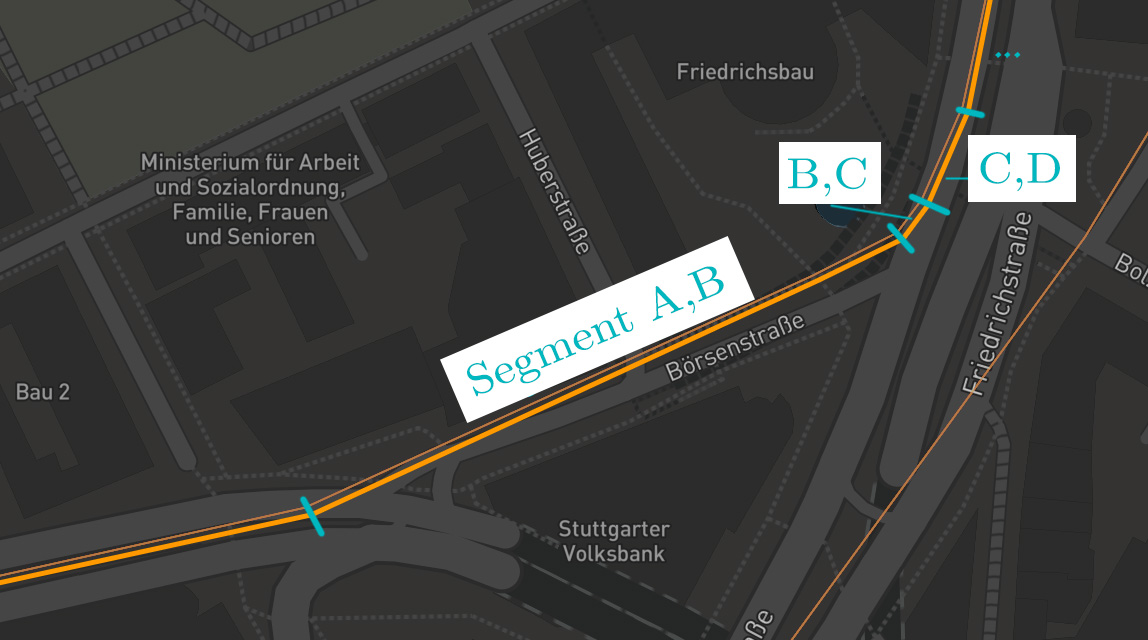
\includegraphics[width=0.45\textwidth]{polyline_segments}
        \caption{Polyline Segmente}
        \label{fig:polyline_segments}
      \end{center}
    \end{figure}

    Das bedeutet, dass die Richtung des Vehicles nicht neu berechnet werden muss, solange es diesem Segment folgt. Erst wenn das Vehicle von Segment $A,B$ auf ein neues Segment $B,C$ übergeht, muss die Richtung neu berechnet werden.

    \item \textbf{Aufteilen der Vehicle in zwei Gruppen:} Da der User durch seinen Bildschirm meistens nur einen Teil der Vehicle zu sehen bekommt, sind die Vehicle in die Gruppen unterteilt. Namentlich seien sie als \texttt{Innerhalb} und \texttt{Außerhalb} benannt. Die Gruppe Innerhalb besitzt all diejenigen Vehicle, die sich im Sichtfeld des Anwenders befinden. Diese werden bei der Animation bevorzugt behandelt und erhalten die volle Rechenleistung. Die Gruppe Außerhalb liegt nicht im Sichtfelds und wird maximal jede Sekunde nach ihrer Aktivität geprüft. Dadurch bleibt auch diese Gruppe immer aktuell.    
   
  \end{itemize}

% subsubsection verbesserung_der_client_performance (end)